%!TEX program = xelatex
% 完整编译: xelatex -> biber/bibtex -> xelatex -> xelatex
\documentclass[lang=cn,11pt,a4paper]{elegantpaper}

\usepackage{algorithm}
\usepackage[noend]{algpseudocode}
\usepackage{amsmath}
\usepackage{array}
\usepackage{xcolor}
\usepackage{graphicx}

\lstdefinelanguage{text}{
    showstringspaces=false,
    breaklines=true,
    breakautoindent=true,
    breakindent=0em,
    tabsize=4
}

\title{《算法设计与分析》\\课程实验报告}

\author{
\huge 专业:计算机科学与技术 \\[10pt]
\huge 班级:2021211304 \\[10pt]
\huge 姓名:杨晨 \\[10pt]
\huge 学号:2021212171
}
\date{}

% 本文档命令
\usepackage{array}
\newcommand{\ccr}[1]{\makecell{{\color{#1}\rule{1cm}{1cm}}}}

\begin{document}

\maketitle

\clearpage

% \begin{abstract}
% 本文为 \href{https://github.com/ElegantLaTeX/ElegantPaper/}{ElegantPaper} 的说明文档。此模板基于 \LaTeX{} 的 article 类,专为工作论文写作而设计。设计这个模板的初衷是让作者不用关心工作论文的格式,专心写作,从而有更加舒心的写作体验。如果你有其他问题、建议或者报告 bug,可以在 \href{https://github.com/ElegantLaTeX/ElegantPaper/issues}{GitHub::ElegantPaper/issues} 留言。如果你想了解更多 Elegant\LaTeX{} 项目组设计的模板,请访问 \href{https://github.com/ElegantLaTeX/}{GitHub::ElegantLaTeX}。
% \keywords{Elegant\LaTeX{},工作论文,模板}
% \end{abstract}


\section{概述}

\subsection{实验内容}

\begin{itemize}
    \item 编程实现下述2组算法之一(二选一), 并利用给定的数据,验证算法正确性
    \begin{itemize}
        \item 第一组
        \begin{itemize}
            \item 最长公共子序列
            \item 最大子段和
        \end{itemize}
        \item 第二组
        \begin{itemize}
            \item 凸多边形最优三角剖分
        \end{itemize}
        \item 动态规划法求最优解,启发式/贪心策略求次优解
    \end{itemize}
\end{itemize}

\subsection{开发环境}

\begin{itemize}
    \item Windows10
    \item PyCharm 2023.2.4 (Professional Edition)
    \item Visual Studio Code 1.84.2
\end{itemize}

\section{实验过程}

\subsection{最长公共子序列}

\subsubsection{介绍}
最长公共子序列(Longest Common Subsequence,简称LCS)问题是计算机科学中的经典问题,在DNA序列对比、文本比较和版本控制系统等领域都有应用。给定两个序列,目标是找到在两个序列中都出现的最长子序列,该子序列不一定是连续的。


\subsubsection{算法描述}

使用动态规划方法解决最长公共子序列(LCS)问题。首先,定义两个输入序列 $X$ 和 $Y$,其中 $X$ 的长度为 $m$,$Y$ 的长度为 $n$。使用一个二维数组 $dp$ 来存储中间结果,其中 $dp[i][j]$ 表示序列 $X$ 的前 $i$ 个元素和序列 $Y$ 的前 $j$ 个元素的最长公共子序列的长度。

算法的核心思想是通过填充 $dp$ 数组来逐步构建最长公共子序列。使用另一个二维数组 $path$ 来记录填充 $dp$ 数组时的选择路径,以便在最后构建最长公共子序列时进行回溯。

具体而言,按照以下步骤执行算法:

\begin{enumerate}
  \item 初始化 $dp$ 和 $path$ 数组为大小为 $(m+1) \times (n+1)$ 的二维数组,并将所有元素初始化为 $0$。
  \item 使用双重循环遍历序列 $X$ 和序列 $Y$ 的所有元素:
    \begin{itemize}
      \item 如果 $X[i]$ 等于 $Y[j]$,则说明当前元素是公共子序列的一部分,因此将 $dp[i][j]$ 更新为 $dp[i-1][j-1] + 1$,并将 $path[i][j]$ 设置为 $1$,表示选择该元素。
      \item 否则,比较 $dp[i-1][j]$ 和 $dp[i][j-1]$ 的值:
        \begin{itemize}
          \item 如果 $dp[i-1][j]$ 大于等于 $dp[i][j-1]$,则说明选择 $X$ 的第 $i$ 个元素作为公共子序列的一部分,将 $dp[i][j]$ 更新为 $dp[i-1][j]$,并将 $path[i][j]$ 设置为 $2$。
          \item 否则,选择 $Y$ 的第 $j$ 个元素作为公共子序列的一部分,将 $dp[i][j]$ 更新为 $dp[i][j-1]$,并将 $path[i][j]$ 设置为 $3$。
        \end{itemize}
    \end{itemize}
  \item 最后,通过对 $path$ 数组进行回溯,可以构建得到最长公共子序列。
\end{enumerate}

\begin{algorithm}[H]
\caption{递归输出LCS}
\begin{algorithmic}[1]
\Procedure{LCS}{$i, j, X, path$}
    \If{$i = 0$ or $j = 0$}
        \State \textbf{return}
    \EndIf
    \If{$path[i][j] = 1$}
        \State \textsc{LCS}($i - 1, j - 1, X, path$)
        \State \textsc{print}($X[i]$)
    \ElsIf{$path[i][j] = 2$}
        \State \textsc{LCS}($i - 1, j, X, path$)
    \Else
        \State \textsc{LCS}($i, j - 1, X, path$)
    \EndIf
\EndProcedure
\end{algorithmic}
\end{algorithm}

\begin{algorithm}[H]
\caption{LCSLength算法}
\begin{algorithmic}[1]
\Procedure{LCSLength}{$X, Y$}
    \State $m \gets \text{length of } X$
    \State $n \gets \text{length of } Y$
    \State $dp \gets \text{new int array of size } (m + 1) \times (n + 1)$ \Comment{初始化为0}
    \State $path \gets \text{new int array of size } (m + 1) \times (n + 1)$ \Comment{初始化为0}
    \For{$i \gets 1$ to $m$}
        \For{$j \gets 1$ to $n$}
            \If{$X[i] = Y[j]$}
                \State $dp[i][j] \gets dp[i - 1][j - 1] + 1$
                \State $path[i][j] \gets 1$
            \ElsIf{$dp[i - 1][j] \geq dp[i][j - 1]$}
                \State $dp[i][j] \gets dp[i - 1][j]$
                \State $path[i][j] \gets 2$
            \Else
                \State $dp[i][j] \gets dp[i][j - 1]$
                \State $path[i][j] \gets 3$
            \EndIf
        \EndFor
    \EndFor
    \State \textsc{LCS}($m, n, X, path$)
\EndProcedure
\end{algorithmic}
\end{algorithm}

\subsubsection{分析和改进}
LCS 算法的时间复杂度为 $O(m \times n)$,其中 $m$ 和 $n$ 分别是序列 $X$ 和序列 $Y$ 的长度。算法需要填充一个大小为 $(m+1) \times (n+1)$ 的二维数组,并进行双重循环遍历。空间复杂度也为 $O(m \times n)$,用于存储 $dp$ 和 $path$ 数组。

在分析代码时,注意到以下改进的可能性:

空间复杂度优化: 给定代码中使用了一个大小为 $(n+1)*(m+1)$ 的一维数组 dp 来存储动态规划的结果。然而,实际上在每次迭代中,只需要使用 dp[i][j]、dp[i][j - 1] 和 dp[i - 1][j - 1] 这三个变量。因此,如果只计算长度的话,可以使用一维数组。这样可以将空间复杂度从 $O(m \times n)$ 优化为 $O(n)$。

空间复杂度优化后的伪代码如下:

\begin{algorithm}[h]
\caption{计算最长公共子序列长度(空间复杂度O(n))}
\begin{algorithmic}[1]
\Procedure{LCS\_Spacesaving}{$X, Y$}
    \State $m \gets \text{length of }(X)$
    \State $n \gets \text{length of }(Y)$
    \State $dp \gets \text{新数组}(n + 1)$
    \For{$i \gets 0$ to $n$}
        \State $dp[i] \gets 0$
    \EndFor
    \For{$i \gets 1$ to $m$}
        \State $\text{upLeft} \gets dp[0]$ \Comment{保存左上角的值}
        \For{$j \gets 1$ to $n$}
            \State $\text{temp} \gets dp[j]$ \Comment{保存当前位置的值,即$dp[i-1][j]$,因为$dp[j]$已经被更新了}
            \If{$X[i] = Y[j]$}
                \State $dp[j] \gets \text{upLeft} + 1$
            \Else
                \State $dp[j] \gets \text{Max}(dp[j], dp[j - 1])$
            \EndIf
            \State $\text{upLeft} \gets \text{temp}$ \Comment{更新左上角的值}
        \EndFor
    \EndFor
\EndProcedure
\end{algorithmic}
\end{algorithm}

\subsubsection{运行结果}
\begin{lstlisting}[language=text]
A and B LCS:
an+algorithm+is+any+welldefined+computational+procedure+that+takes+some+values+as+input+and+produces+some+values+as+output20212113xx2023
LCSLength is: 137
LCSLength is: 137

A and C LCS:
an+algorithm+is+any+welldefined+computational+procedure+that+takes+some+values+as+input+and+produces+some+values+as+output20212113xx2023
LCSLength is: 137
LCSLength is: 137

A and D LCS:
an+algorithm+is+any+welldefined+computational+procedure+that+takes+some+values+as+input+and+produces+some+values+as+output20212113xx2023
LCSLength is: 137
LCSLength is: 137

C and B LCS:
an+algorithm+is+any+welldefined+computational+procedure+that+takes+some+values+as+input+and+produces+some+values+as+output20212113xx2023
LCSLength is: 137
LCSLength is: 137
\end{lstlisting}

\subsubsection{结论}
LCS 算法提供了一种有效的方法来寻找两个序列中的最长公共子序列。通过动态规划的思想,算法能够在较快的时间内计算出最长公共子序列的长度,并通过回溯路径构建得到最长公共子序列。如果不需要得到具体的序列,空间复杂度可以优化为O(n)。

\subsection{最长不上升子序列}

\subsubsection{介绍}
最长不上升子序列(Longest Decreasing Subsequence,简称LDS)是指在给定序列中找到最长的子序列,使得子序列中的元素按照非递增的顺序排列。LDS问题在计算机科学和算法设计中具有重要意义,广泛应用于数据分析、信号处理、优化问题等领域。

\subsubsection{算法描述}

首先介绍一种基于最长公共子序列的方法,来求解最长不上升子序列问题的算法。

借助最长公共子序列(LCS)的思想来解决最长不上升子序列问题首先,将原始序列保存在$num\_temp$中,并对$num$进行非递增排序,得到新的序列。然后,使用动态规划的方法计算最长公共子序列的长度和路径。最后,根据路径信息输出最长不上升子序列。

下面是借助最长公共子序列(LCS)求解最长不上升子序列问题的算法的伪代码:

\begin{algorithm}[H]
\caption{借助最长公共子序列求最长不上升子序列}
\begin{algorithmic}[1]
\Procedure{LDS\_by\_LCS}{$\text{num}: \text{vector<int>}$}
    \State $n \gets \text{num.size()}$
    \State $\text{num\_temp} \gets \text{num}$
    \State $\text{sort}(\text{num.begin()}, \text{num.end()}, \text{greater<int>()})$ \Comment{以降序排序}
    \State $\text{dp} \gets \text{vector<vector<int>>(n + 1, vector<int>(n + 1, 0))}$
    \State $\text{path} \gets \text{vector<vector<int>>(n + 1, vector<int>(n + 1, 0))}$
    \For{$i \gets 1$ to $n$}
        \For{$j \gets 1$ to $n$}
            \If{$\text{num}[i - 1] = \text{num\_temp}[j - 1]$}
                \State $\text{dp}[i][j] \gets \text{dp}[i - 1][j - 1] + 1$
                \State $\text{path}[i][j] \gets 1$
            \ElsIf{$\text{dp}[i - 1][j] \geq \text{dp}[i][j - 1]$}
                \State $\text{dp}[i][j] \gets \text{dp}[i - 1][j]$
                \State $\text{path}[i][j] \gets 2$
            \Else
                \State $\text{dp}[i][j] \gets \text{dp}[i][j - 1]$
                \State $\text{path}[i][j] \gets 3$
            \EndIf
        \EndFor
    \EndFor
    \State \textbf{printf} "最长不上升子序列长度为:" + $\text{dp}[n][n]$
    \State \textbf{printf} "最长不上升子序列为:"
    \Procedure{output}{$i: \text{int}$, $j: \text{int}$}
        \If{$i = 0$ or $j = 0$}
            \State \textbf{return}
        \EndIf
        \If{$\text{path}[i][j] = 1$}
            \State \textbf{output} $(i - 1, j - 1)$
            \State \textbf{printf} $\text{num}[i - 1]$
        \ElsIf{$\text{path}[i][j] = 2$}
            \State \textbf{output} $(i - 1, j)$
        \Else
            \State \textbf{output} $(i, j - 1)$
        \EndIf
    \EndProcedure
    \State \textbf{output} $(n, n)$
\EndProcedure
\end{algorithmic}
\end{algorithm}

此外,还可以使用动态规划的思想来解决最长不上升子序列问题。首先,定义一个长度为$n$的数组$dp$,其中$dp[i]$表示以序列中第$i$个元素结尾的最长不上升子序列的长度。初始化$dp$数组的所有元素为1,表示每个元素本身就构成一个长度为1的子序列。

然后,通过两层循环遍历序列中的每个元素,比较当前元素和前面已经遍历过的元素的大小关系。如果当前元素小于等于前面的元素,并且以前面元素结尾的子序列的长度加1大于以当前元素结尾的子序列的长度,则更新$dp$数组和路径数组$path$。

最后,遍历$dp$数组找到最长的子序列长度和对应的索引,根据路径数组$path$逆序输出最长不上升子序列的元素。

下面是基于动态规划的最长不上升子序列算法的伪代码:

\begin{algorithm}[H]
\caption{最长不上升子序列}
\begin{algorithmic}[1]
\Procedure{LDS}{num: vector<int>}
    \State $n \gets \text{num.size()}$
    \State $dp \gets \text{vector<int>(n, 1)}$ // dp[i]表示以num[i]结尾的最长不上升子序列的长度
    \State $path \gets \text{vector<int>(n, -1)}$
    \For{$i \gets 1$ to $n-1$}
    \For{$j \gets 0$ to $i-1$}
    \If{$\text{num}[i] \leq \text{num}[j]$ and $\text{dp}[i] < \text{dp}[j] + 1$}
    \State $\text{dp}[i] \gets \text{dp}[j] + 1$
    \State $\text{path}[i] \gets j$
    \EndIf
    \EndFor
    \EndFor
    \State $ans \gets \text{dp}[0]$
    \State $index \gets 0$
    \For{$i \gets 0$ to $n-1$}
    \If{$\text{ans} < \text{dp}[i]$}
    \State $\text{ans} \gets \text{dp}[i]$
    \State $\text{index} \gets i$
    \EndIf
    \EndFor
    \State \textbf{printf} "最长不上升子序列长度为:" + $\text{ans}$
    \State \textbf{printf} "最长不上升子序列为:"
    \Procedure{output}{$x: \text{int}$} \Comment{匿名函数,定义了一个输出函数}
        \If{$x = -1$}
        \State \textbf{return}
        \EndIf
        \State \textbf{output} $\text{path}[x]$
        \State \textbf{printf} $\text{num}[x]$
    \EndProcedure
    \State \textbf{output} $\text{index}$
\EndProcedure
\end{algorithmic}
\end{algorithm}

\subsubsection{分析和改进}
第一个算法的时间复杂度为$O(n^2)$,空间复杂度为$O(n^2)$,其中$n$是序列的长度。算法使用了一个二维数组$dp$来保存最长公共子序列的长度,以及一个二维数组$path$来保存路径信息。在输出最长不上升子序列时,使用了递归函数$output$来回溯路径并输出结果。

第二个算法的时间复杂度为$O(n^2)$,但是空间复杂度降为了$O(n)$,其中$n$是序列的长度。算法使用了一个一维数组$dp$来保存最长公共子序列的长度,以及一个一维数组$path$来保存路径信息。在输出最长不上升子序列时,使用了递归函数$output$来回溯路径并输出结果。

当然,如果只找最长不上升序列的长度,时间复杂度还可以进一步降低。将原来的dp数组的存储由数值换成该序列中,不上升子序列长度为i的序列中的,最大的末尾数值

这其实就是一种几近贪心的思想:当前的不上升子序列长度如果已经确定,那么如果这种长度的子序列的结尾元素越大,后面的元素就可以更方便地加入到这条我们臆测的、可作为结果、的不上升子序列中。

伪代码如下:
\begin{algorithm}[H]
\caption{计算最长不上升子序列的长度(时间复杂度 O(nlogn))}
\begin{algorithmic}[1]
\Procedure{LDS\_nlogn}{$\text{num}: \text{vector<int>}$}
    \State $n \gets \text{num.size()}$
    \State $\text{dp} \gets \text{vector<int>(n + 1, INT\_MAX)}$ \Comment{dp[i]表示长度为i的最长不上升子序列的最大末尾元素}
    \State $len \gets 0$
    \For{$i \gets 0$ to $n - 1$}
        \If{$\text{num}[i] \leq \text{dp}[len]$} \Comment{如果num[i]≤最长不上升子序列的最大末尾元素,那么num[i]可以接在最长不上升子序列后面,形成一个更长的不上升子序列}
            \State $len \gets len + 1$
            \State $\text{dp}[len] \gets \text{num}[i]$
        \Else \Comment{否则,找到dp中第一个小于num[i]的元素,用num[i]替换它}
            \State $pos \gets \text{upper\_bound}(\text{dp.begin()} + 1, \text{dp.begin()} + len + 1, \text{num}[i], \text{greater<int>()}) - \text{dp.begin()}$
            \State $\text{dp}[pos] \gets \text{num}[i]$
        \EndIf
    \EndFor
    \State \textbf{printf} "最长不上升子序列长度为:" + $len$
\EndProcedure
\end{algorithmic}
\end{algorithm}

第三个算法的时间复杂度为$O(n\log n)$,其中$n$是序列的长度。算法通过遍历输入序列并维护一个长度为$L$的数组$\text{dp}$,其中$L$是当前最长不上升子序列的长度。在遍历过程中,算法通过二分查找找到合适的位置,将当前元素插入$\text{dp}$数组中。最后,$\text{dp}$数组的长度即为最长不上升子序列的长度。需要注意的是,dp数组中的元素不是真正的不上升子序列。

\subsubsection{运行结果}
\begin{lstlisting}[language=text]
num1:
最长不上升子序列长度为:40
最长不上升子序列为:99 99 95 93 89 87 87 79 76 72 68 68 68 60 56 51 50 47 36 31 27 27 27 19 3 0 0 0 -4 -10 -14 -15 -17 -22 -27 -57 -100 -211 -301 -305
最长不上升子序列长度为:40
最长不上升子序列为:99 99 95 91 89 87 87 79 76 72 65 61 60 56 56 51 50 47 36 31 27 27 27 19 3 0 0 0 -4 -10 -14 -15 -17 -22 -31 -100 -200 -230 -301 -305
最长不上升子序列长度为:40

num2:
最长不上升子序列长度为:30
最长不上升子序列为:100 49 47 47 39 38 37 34 34 34 33 28 27 24 24 22 10 8 -10 -11 -16 -25 -32 -38 -39 -42 -44 -70 -304 -307
最长不上升子序列长度为:30
最长不上升子序列为:100 49 47 47 39 38 37 34 34 34 33 28 27 24 24 5 -2 -6 -10 -11 -25 -25 -32 -38 -41 -42 -44 -70 -304 -307
最长不上升子序列长度为:30
\end{lstlisting}

\subsubsection{结论}
通过使用转化为最长公共子序列或者动态规划,可以在给定序列中找到最长的不上升子序列。算法的复杂度为$O(n^2)$,其中$n$是序列的长度。

但是,如果只寻找最长不上升子序列的长度,时间复杂度可以进一步降低为$O(n \log n)$。同时,也论证了一个观点:时间复杂度越高的算法越全能。

通过分析和实验,发现该算法可以有效地解决最长不上升子序列问题,并且在实际应用中具有较好的性能。然而,当序列长度非常大时,该算法的时间复杂度可能变得较高,因此在处理大规模数据时需要考虑其他优化方法。

\subsection{最大子段和}

\subsubsection{介绍}
最大子段和问题是一个经典的算法问题,其目标是在给定的整数数组中找到一个连续子数组,使得该子数组的和最大。这个问题在计算机科学和算法设计中具有重要意义,可以应用于许多实际问题,如股票交易、财务分析等领域。
\subsubsection{算法描述}

首先,介绍基于分治法的最大子段和算法。基于分治法,将问题分解为更小的子问题,并通过递归求解子问题来获得最终的解。下面是伪代码:

\begin{algorithm}[H]
\caption{最大子段和算法}
\begin{algorithmic}[1]
\Function{MaxSubSum}{$num, left, right$}
    \If{$left = right$}
    \State \Return $num[left] > 0 ? num[left] : 0$
    \EndIf
    \State $mid \gets (left + right) / 2$
    \State $leftMax \gets \text{MaxSubSum}(num, left, mid)$
    \State $rightMax \gets \text{MaxSubSum}(num, mid + 1, right)$
    \State $leftBorderMax \gets num[mid]$
    \State $leftBorderSum \gets 0$
    \For{$i \gets mid$ \textbf{downto} $left$}
    \State $leftBorderSum \gets leftBorderSum + num[i]$
    \If{$leftBorderSum > leftBorderMax$}
    \State $leftBorderMax \gets leftBorderSum$
    \EndIf
    \EndFor
    \State $rightBorderMax \gets num[mid + 1]$
    \State $rightBorderSum \gets 0$
    \For{$i \gets mid + 1$ \textbf{to} $right$}
    \State $rightBorderSum \gets rightBorderSum + num[i]$
    \If{$rightBorderSum > rightBorderMax$}
    \State $rightBorderMax \gets rightBorderSum$
    \EndIf
    \EndFor
    \State $borderMax \gets leftBorderMax + rightBorderMax$
    \State \Return $\max(\max(leftMax, rightMax), borderMax)$
\EndFunction
\State
\Function{MaxSubSum}{$num$} \Comment{重载隐藏参数}
    \State \Return \text{MaxSubSum}($num, 0, \text{size}(num) - 1$)
\EndFunction
\end{algorithmic}
\end{algorithm}

\subsubsection{分析与改进}

在之前的报告中,介绍了基于分治法的最大子段和算法。下面将介绍一种改进后的算法,基于动态规划思想,来解决最大子序列和问题。

改进后的最大子序列和算法基于动态规划思想,使用一个变量$dp$来记录当前位置的最大子序列和。算法从数组的第二个元素开始遍历,若$dp$大于零,则将当前元素加到$dp$上;否则,将$dp$更新为当前元素,并更新最大子序列的起始位置,因为负数对后边的序列是无用的。在遍历的过程中,不断更新最大子序列和$ans$和最大子序列的终止位置$right$。

下面是改进后的最大子序列和算法的伪代码:

\begin{algorithm}[H]
\caption{最大子序列和改进算法}
\begin{algorithmic}[1]
\Procedure{MaxSum}{$num$}
    \State $n \gets \text{size}(num)$
    \State $dp \gets num[0]$
    \State $ans \gets num[0]$
    \State $left \gets 0$
    \State $right \gets 0$
    \For{$i \gets 1$ \textbf{to} $n-1$}
    \If{$dp > 0$}
    \State $dp \gets dp + num[i]$
    \Else
    \State $dp \gets num[i]$
    \State $left \gets i$
    \EndIf
    \If{$dp > ans$}
    \State $ans \gets dp$
    \State $right \gets i$
    \EndIf
    \EndFor
    \State \textbf{printf} "最大子序列和为:" $ans$
    \State \textbf{printf} "最大子序列为:"
    \For{$i \gets left$ \textbf{to} $right$}
    \State \textbf{printf} $num[i]$
    \EndFor
\EndProcedure
\end{algorithmic}
\end{algorithm}

\subsubsection{运行结果}
\begin{lstlisting}[language=text]
num1最大子段和为: 6914
num1最大子序列和为:6914
最大子序列为:64 87 99 39 31 9 99 -2 -7 83 -46 8 16 55 -88 31 -96 51 -60 90 -13 80 50 -88 -9 -84 95 68 -23 24 53 -94 91 60 -34 -19 -53 -40 13 -31 -35 70 25 38 65 49 -99 68 -18 17 79 70 11 -93 93 -24 13 74 70 20 -2 66 97 -20 -56 89 5 -86 87 -56 53 60 73 15 -83 -73 -11 59 -85 87 -24 -81 79 70 -12 29 -4 63 -58 -48 94 20 -68 -10 76 97 72 -56 -45 -96 3 53 60 13 97 65 22 78 99 -12 68 -13 24 -73 -89 22 61 -31 73 5 27 81 -85 55 68 -56 43 60 -19 -23 77 -91 -61 -57 22 -39 -64 29 41 -15 -43 -43 -4 -47 49 -21 66 0 56 45 71 -16 -35 68 60 -26 98 -22 -62 56 51 -63 -83 -62 -48 -33 9 11 5 57 93 35 32 -80 -54 -87 -82 -96 39 93 -89 50 29 47 7 -13 80 23 -85 -38 3 25 36 31 92 46 82 -23 -46 91 89 -40 76 -12 53 -88 -74 27 49 14 42 -60 -32 -43 -18 65 -57 27 27 46 68 -29 63 84 -9 40 -42 -4 -32 -35 82 19 35 -15 84 76 -28 -42 -99 39 79 -54 -9 98 -77 95 -82 -60 -86 3 0 -85 70 -80 33 0 57 73 94 -50 -91 -46 0 42 -98 43 68 -18 -4 25 32 65 -29 -62 -76 78 12 -30 -10 61 94 92 -67 20 -51 33 95 -97 -94 -14 68 31 -15 -55 19 23 -44 25 -17 -48 45 72 37 -22 48 -31 -27 82 16 -20 30 -100 -200 50 60 300 -2 8 -230 45 78 -69 54 29 300 -57 63 70 -120 80 -100 40 20 30 2021 -211 -301 304 -305 307 2023

num2最大子段和为: 2583
num2最大子序列和为:2583
最大子序列为:34 1 -5 40 8 2 6 23 30 42 -4 45 -25 -23 -22 34 -13 -11 -12 16 44 -3 -11 -7 -30 34 49 -47 1 -21 -37 14 33 -37 28 -33 15 -36 36 27 -8 -31 24 -16 -7 38 24 34 48 -27 -22 5 33 9 -26 -2 48 -20 22 38 -42 4 5 -49 10 47 -6 27 8 -10 34 -11 -25 -35 -17 38 43 -9 -8 -16 -25 -32 10 -38 -41 -18 -1 37 1 25 -39 -35 10 -23 -23 -20 43 -4 -42 -9 44 26 -16 41 -1 20 -33 50 -100 130 32 -99 2 -44 36 -15 80 8 15 -15 31 10 20 -40 60 -70 20 30 40 -21 211 301 -304 305 -307 2023
\end{lstlisting}
\subsubsection{结论}
基于分治的算法的时间复杂度为$O(n\log n)$,其中$n$是输入数组的大小。这是因为在每次递归调用中,问题的规模减少一半,而对于每个子问题,需要线性时间来计算边界最大和。因此,总体的时间复杂度为$O(n\log n)$。

基于动态规划的算法的时间复杂度为$O(n)$,其中$n$是输入数组的大小。

\subsection{凸多边形最优三角剖分}

\subsubsection{介绍}
凸多边形最优三角剖分问题是计算机图形学中的一个经典问题,其目标是在给定的凸多边形中找到一种三角剖分方式,使得剖分后的三角形的权值之和最小。

\subsubsection{算法描述}
凸多边形最优三角剖分算法基于动态规划思想,通过填表的方式求解最优解。算法维护一个二维数组$dp$,其中$dp[i][j]$表示从第$i$个顶点到第$j$个顶点的最优三角剖分的最小权值。同时,算法还维护一个二维数组$s$,用于记录最优三角剖分对应的顶点。算法从小到大枚举区间长度,然后从左端点开始枚举,计算每个区间的最优三角剖分权值,并更新$dp$和$s$数组。最后,调用$draw\_stations$函数将最优三角剖分可视化。



下面是凸多边形最优三角剖分问题的动态规划算法的伪代码:

\begin{algorithm}[H]
\caption{凸多边形最优三角剖分算法}
\begin{algorithmic}[1]
\Procedure{OptimalTriangulation}{stations}
    \State $n \gets \text{len}(stations)$
    \State $dp \gets [[0 \text{ for } \_ \text{ in range}(n)] \text{ for } \_ \text{ in range}(n)]$ \Comment{n $\times$ n二维列表,初始化为0}
    \State $s \gets [[0 \text{ for } \_ \text{ in range}(n)] \text{ for } \_ \text{ in range}(n)]$ \Comment{n $\times$ n二维列表,初始化为0}
    \For{$i \text{ in range}(n - 1)$}
        \State $dp[i][i + 1] \gets 0$
    \EndFor
    \For{$\text{len\_} \text{ in range}(3, n + 1)$}
        \For{$l \text{ in range}(n - \text{len\_} + 1)$}
            \State $r \gets l + \text{len\_} - 1$
            \State $dp[l][r] \gets \text{极大值}$
            \For{$k \text{ in range}(l + 1, r)$}
                \If{$dp[l][r] > dp[l][k] + dp[k][r] + weight$}
                    \State $dp[l][r] \gets dp[l][k] + dp[k][r] + weight$
                    \State $s[l][r] \gets k$
                \EndIf
            \EndFor
        \EndFor
    \EndFor
    \State \textbf{调用} $draw\_stations(stations, s)$ \Comment{画图展示最优三角剖分}
    \State \textbf{print} $dp[0][n - 1]$
\EndProcedure
\end{algorithmic}
\end{algorithm}

\subsubsection{分析和改进}
凸多边形最优三角剖分算法的时间复杂度主要取决于两个嵌套的循环:外层循环枚举区间长度,内层循环枚举左端点。对于给定的区间长度,内层循环的迭代次数是固定的,取决于区间长度。因此,算法的时间复杂度可以表示为$O(n^3)$,其中,$n$是凸多边形的顶点数。在内层循环中,还进行了常数次的计算和更新操作,它们的时间复杂度可以忽略不计。

因此,凸多边形最优三角剖分算法的时间复杂度为$O(n^3)$,在顶点数较小的情况下,算法能够在合理的时间范围内求解最优三角剖分问题。

在点的数量比较大时,采用$O(n^3)$的算法会花费较多的时间。下面将提出一种凸多边形最优三角剖分问题的近似算法,该算法采用了贪心策略和随机选择的方法。首先,算法初始化了一些必要的变量和数据结构。然后,从小到大枚举区间长度和左端点,利用随机选择的 $k$ 个分割点对权值进行近似计算。在计算过程中,算法根据当前的最优解更新策略来更新最小权值和对应的分割点。最后,算法输出凸多边形的最优三角剖分的最小权值。

该算法的时间复杂度为 $O(n^3)$,其中 $n$ 是基站列表的长度。算法中的两个嵌套循环分别对应了区间长度和左端点的枚举,因此需要 $O(n^2)$ 的时间复杂度。在每个区间和左端点的循环中,算法通过随机选择的 $k$ 个分割点对权值进行近似计算,这需要 $O(k)$ 的时间复杂度。因此,总的时间复杂度为 $O(n^2 \cdot k)$,由于$k \leq 5$,所以时间复杂度为$O(n^2)$

下面是凸多边形最优三角剖分问题的近似算法的伪代码:

\begin{algorithm}[H]
\caption{凸多边形最优三角剖分近似算法}
\begin{algorithmic}[1]
\Procedure{OptimalTriangulationApprox}{stations, k}
    \State $n \gets \text{len}(stations)$
    \State $dp \gets [[0 \text{ for } \_ \text{ in range}(n)] \text{ for } \_ \text{ in range}(n)]$ \Comment{n $\times$ n二维列表,初始化为0}
    \State $s \gets [[0 \text{ for } \_ \text{ in range}(n)] \text{ for } \_ \text{ in range}(n)]$ \Comment{n $\times$ n二维列表,初始化为0}
    \For{$i \text{ in range}(n - 1)$}
        \State $dp[i][i + 1] \gets 0$
    \EndFor
    \For{$\text{len\_} \text{ in range}(3, n + 1)$}
        \For{$l \text{ in range}(n - \text{len\_} + 1)$}
            \State $r \gets l + \text{len\_} - 1$
            
            \Comment{贪心策略,直接从随机选择的k个分割点中选取最好的分割点,范围[l+1,r-1]}
            \If{$r - l - 1 > k$}
                \State $split\_points \gets \text{random\_choice}(\{l + 1, l + 2, ..., r - 1\}, k, \text{replace}=\text{False})$
            \Else \Comment{如果区间长度小于等于k,则选取所有的分割点}
                \State $split\_points \gets \{l + 1, l + 2, ..., r - 1\}$
            \EndIf
            \For{$k \text{ in } \text{split\_points}$}
                \If{$dp[l][r] == 0 \text{ or } dp[l][r] > dp[l][k] + dp[k][r] + weight$}
                    \State $dp[l][r] \gets dp[l][k] + dp[k][r] + weight$
                    \State $s[l][r] \gets k$
                \EndIf
            \EndFor
        \EndFor
    \EndFor
    \State \textbf{调用} $draw\_stations(stations, s, \text{title}=\text{"Optimal Triangulation Approx"})$ \Comment{画图展示最优三角剖分}
    \State \textbf{print} $dp[0][n - 1]$
\EndProcedure
\end{algorithmic}
\end{algorithm}

\subsubsection{运行结果}
\begin{lstlisting}[language=text]
21个基站凸多边形数据
0 19 20
0 7 19
0 6 7
0 1 6
1 5 6
1 2 5
2 4 5
2 3 4
7 8 19
8 18 19
8 9 18
9 17 18
9 13 17
9 12 13
9 11 12
9 10 11
13 16 17
13 15 16
13 14 15
最优三角剖分的最小权值150529.07457599998
0 19 20
0 7 19
0 6 7
0 1 6
1 5 6
1 2 5
2 4 5
2 3 4
7 8 19
8 18 19
8 9 18
9 17 18
9 13 17
9 12 13
9 11 12
9 10 11
13 16 17
13 15 16
13 14 15
最优三角剖分的近似最小权值150529.07457599998
\end{lstlisting}

\begin{figure}[htbp]
\centering
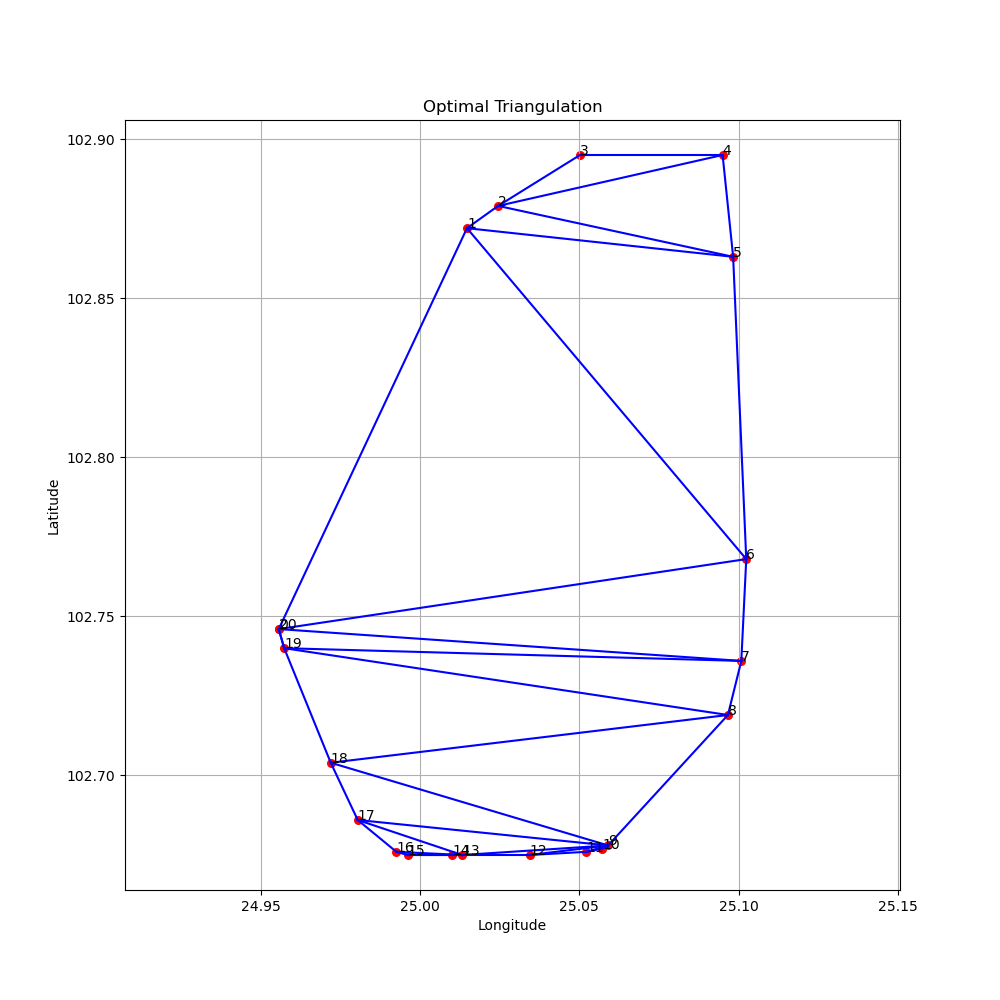
\includegraphics[width=0.8\textwidth, height=0.4\textheight]{image/result1.png}
\caption{21个基站最优解}
\end{figure}

\begin{figure}[htbp]
\centering
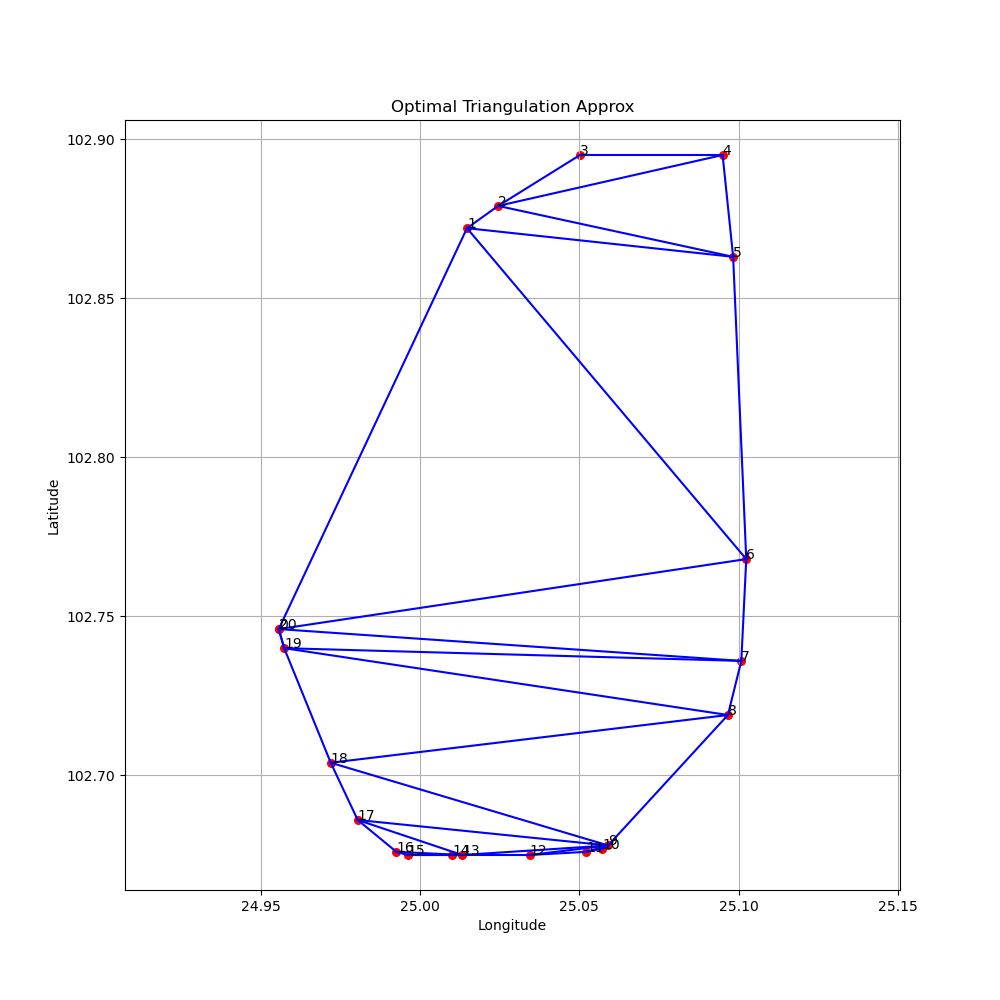
\includegraphics[width=0.8\textwidth, height=0.4\textheight]{image/result2.png}
\caption{21个基站近似解}
\end{figure}

\begin{lstlisting}
29个基站凸多边形数据
0 1 28
1 11 28
1 9 11
1 2 9
2 3 9
3 8 9
3 4 8
4 7 8
4 5 7
5 6 7
9 10 11
11 12 28
12 13 28
13 27 28
13 15 27
13 14 15
15 24 27
15 16 24
16 23 24
16 17 23
17 22 23
17 19 22
17 18 19
19 21 22
19 20 21
24 26 27
24 25 26
最优三角剖分的最小权值93108.00227200001
0 1 28
1 11 28
1 9 11
1 2 9
2 3 9
3 8 9
3 4 8
4 7 8
4 5 7
5 6 7
9 10 11
11 12 28
12 13 28
13 27 28
13 15 27
13 14 15
15 24 27
15 16 24
16 23 24
16 17 23
17 22 23
17 19 22
17 18 19
19 21 22
19 20 21
24 26 27
24 25 26
最优三角剖分的近似最小权值93108.00227200001
\end{lstlisting}

\begin{figure}[!htb]
\centering
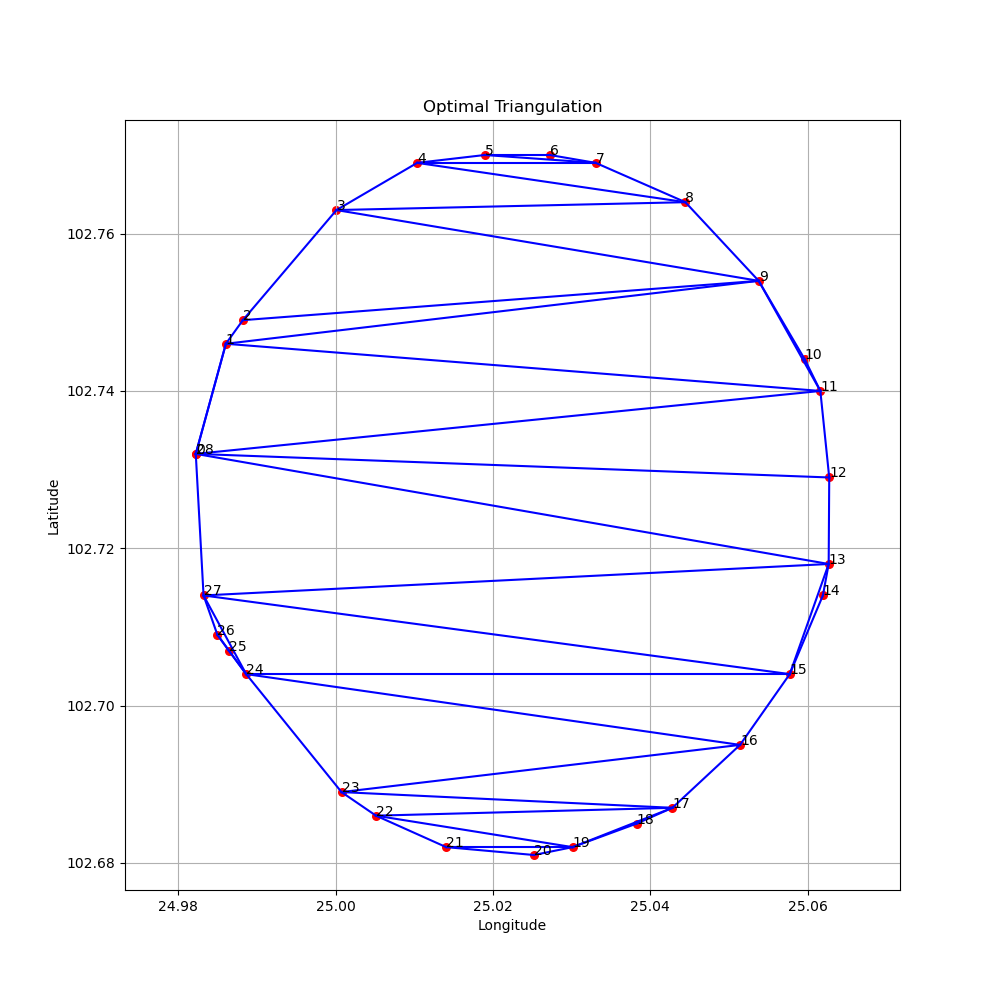
\includegraphics[width=0.8\textwidth, height=0.4\textheight]{image/result3.png}
\caption{29个基站最优解}
\end{figure}

\begin{figure}[!htb]
\centering
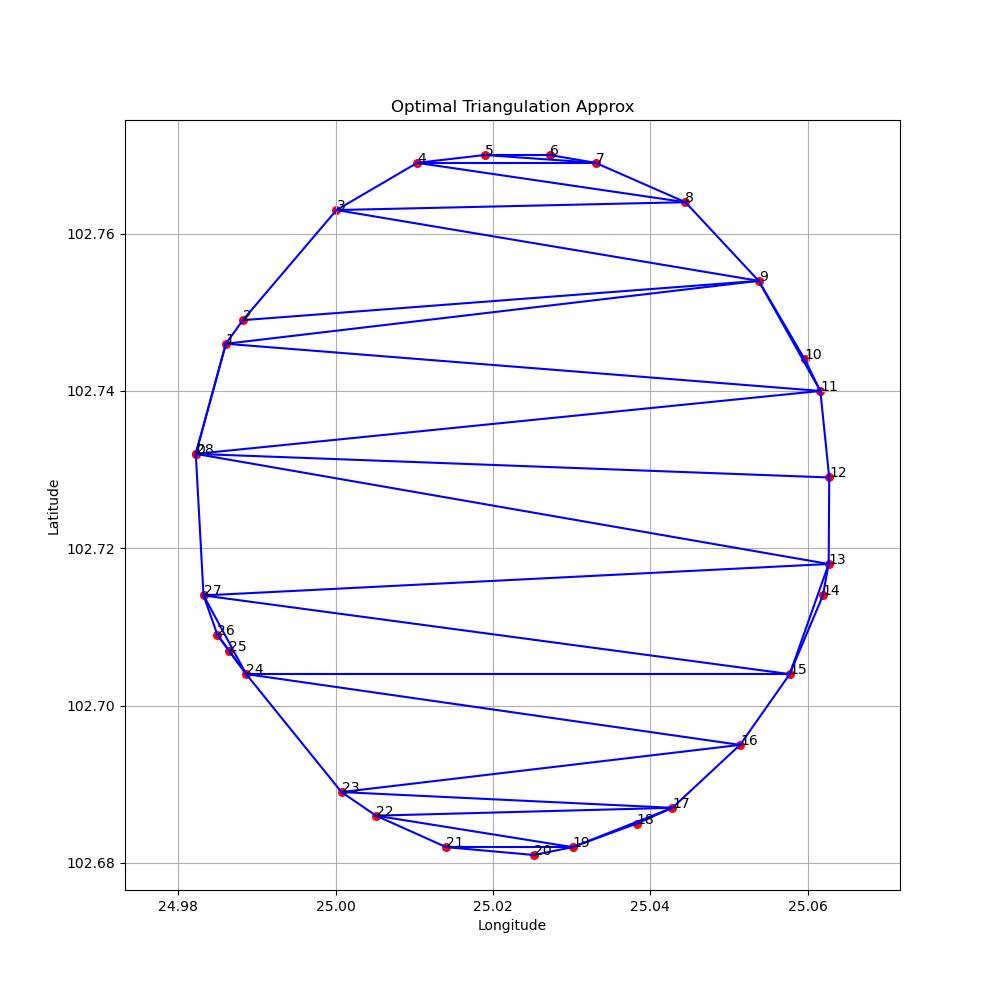
\includegraphics[width=0.8\textwidth, height=0.4\textheight]{image/result4.png}
\caption{29个基站近似解}
\end{figure}

\clearpage

\subsubsection{结论}
凸多边形最优三角剖分问题是一个经典的计算机图形学问题,动态规划算法提供了一种有效的解决方案。通过填表和状态转移的方式,算法可以在$O(n^3)$的时间复杂度内求解最优三角剖分的最小权值。通过对算法的分析和实验结果的验证,可以得出结论:凸多边形最优三角剖分算法能够正确地找到凸多边形的最优三角剖分,使得剖分后的三角形的权值之和最小。

此外,基于近似算法的凸多边形最优三角剖分解法,通过贪心策略和随机选择的方法,近似计算凸多边形的最优三角剖分的最小权值。算法的时间复杂度为 $O(n^2)$,其中 $n$ 是基站列表的长度。通过实验和分析,可以得出该算法在给定的时间复杂度范围内,能够得到较好的近似解。

\subsection{0-1背包问题}

\subsubsection{介绍}
0-1背包问题是一个经典的组合优化问题,它的目标是在给定的一组物品中,选取一些物品放入容量有限的背包中,使得选取的物品总重量不超过背包的容量,并且选取的物品总价值最大化。该问题的名称来源于每个物品只能选择放入背包一次(0表示不放入,1表示放入)的限制条件。

在实际应用中,0-1背包问题有着广泛的应用,例如资源分配、货物装载、投资组合等领域。
\subsubsection{算法描述}
0-1背包问题的算法采用动态规划的方法进行求解。算法的时间复杂度主要取决于物品数量$n$和背包容量$m$。

在算法中,使用一个二维数组$f$来保存前$i$个物品放入容量为$j$的背包中的最大价值。算法的核心部分是两个嵌套的循环,这两个循环分别遍历物品和背包容量,每个内部循环的时间复杂度为$O(1)$。因此,算法的总时间复杂度为$O(nm)$。

以下是解决0-1背包问题的伪代码:

\begin{algorithm}[H]
\caption{0-1背包问题}\label{knapsack}
\begin{algorithmic}[1]
\Procedure{ZeroOneKnapsack}{$capacity, weights, values$}
\State $n \gets$ \Call{Length}{$weights$} \Comment{物品数量}
\State $m \gets capacity$ \Comment{背包容量}
\State $f \gets$ \Call{Create2DArray}{$n+1, m+1$} \Comment{初始化二维数组}
\For{$i \gets 1$ \textbf{to} $n$}
    \For{$j \gets 1$ \textbf{to} $m$}
        \If{$weights[i-1] \leq j$}
            \State $f[i][j] \gets \max(f[i-1][j], f[i-1][j-weights[i-1]] + values[i-1])$
        \Else
            \State $f[i][j] \gets f[i-1][j]$
        \EndIf
    \EndFor
\EndFor

\State $x \gets$ \Call{CreateArray}{$n$} \Comment{初始化最优解列表}
\State $j \gets m$
\For{$i \gets n$ \textbf{downto} $1$}
    \If{$f[i][j] > f[i-1][j]$}
        \State $x[i-1] \gets 1$
        \State $j \gets j - weights[i-1]$
    \EndIf
\EndFor

\State \textbf{return} $f[n][m], x$ \Comment{返回最大价值和最优解}
\EndProcedure
\end{algorithmic}
\end{algorithm}

\subsubsection{分析和改进}
在原始的动态规划算法中,使用一个二维数组$f$来保存前$i$个物品放入容量为$j$的背包中的最大价值。算法的核心部分是两个嵌套的循环,这两个循环分别遍历物品和背包容量,每个内部循环的时间复杂度为$O(1)$。因此,算法的总时间复杂度为$O(nm)$。

在空间复杂度方面,需要额外的二维数组$f$来保存中间结果,其大小为$(n+1) \times (m+1)$。因此,算法的空间复杂度为$O(nm)$。

然而,如果不需要输出具体的物品放入情况,只关心最大的物品总价值,可以进一步优化空间复杂度。优化后的算法只使用一个一维数组$f$来保存背包容量从0到$m$的最大价值。这样,算法的空间复杂度可以降低到$O(m)$。

以下是优化后的伪代码:

\begin{algorithm}[H]
\caption{0-1背包问题(优化后)}\label{knapsack_optimized}
\begin{algorithmic}[1]
\Procedure{ZeroOneKnapsackSavingSpace}{$capacity, weights, values$}
\State $n \gets$ \Call{Length}{$weights$} \Comment{物品数量}
\State $m \gets capacity$ \Comment{背包容量}
\State $f \gets$ \Call{CreateArray}{$m+1$} \Comment{初始化一维数组}
\For{$i \gets 1$ \textbf{to} $n$}
    \For{$j \gets m$ \textbf{downto} $1$}
        \If{$weights[i-1] \leq j$}
            \State $f[j] \gets \max(f[j], f[j-weights[i-1]] + values[i-1])$
        \EndIf
    \EndFor
\EndFor

\State \textbf{return} $f[m]$ \Comment{返回最大价值}
\EndProcedure
\end{algorithmic}
\end{algorithm}

\subsubsection{运行结果}
\begin{lstlisting}[language=text]
第1组, 最大价值为:  1181
第1个物品放入背包中,重量为14, 价值为50
第2个物品放入背包中,重量为11, 价值为72
第4个物品放入背包中,重量为17, 价值为69
第8个物品放入背包中,重量为26, 价值为59
第9个物品放入背包中,重量为10, 价值为49
第17个物品放入背包中,重量为37, 价值为74
第18个物品放入背包中,重量为19, 价值为71
第23个物品放入背包中,重量为13, 价值为63
第24个物品放入背包中,重量为15, 价值为59
第25个物品放入背包中,重量为9, 价值为48
第26个物品放入背包中,重量为10, 价值为41
第32个物品放入背包中,重量为8, 价值为50
第33个物品放入背包中,重量为11, 价值为48
第38个物品放入背包中,重量为8, 价值为51
第43个物品放入背包中,重量为28, 价值为72
第44个物品放入背包中,重量为16, 价值为46
第45个物品放入背包中,重量为9, 价值为41
第49个物品放入背包中,重量为23, 价值为52
第50个物品放入背包中,重量为18, 价值为77
第51个物品放入背包中,重量为38, 价值为89
背包总重量为:  340
最优解正确

第2组, 最大价值为:  1661
第1个物品放入背包中,重量为10, 价值为61
第5个物品放入背包中,重量为33, 价值为61
第6个物品放入背包中,重量为44, 价值为79
第9个物品放入背包中,重量为15, 价值为59
第11个物品放入背包中,重量为12, 价值为30
第22个物品放入背包中,重量为20, 价值为74
第23个物品放入背包中,重量为18, 价值为46
第27个物品放入背包中,重量为28, 价值为51
第31个物品放入背包中,重量为24, 价值为64
第34个物品放入背包中,重量为31, 价值为54
第42个物品放入背包中,重量为26, 价值为54
第49个物品放入背包中,重量为9, 价值为19
第52个物品放入背包中,重量为18, 价值为67
第54个物品放入背包中,重量为42, 价值为73
第55个物品放入背包中,重量为15, 价值为44
第58个物品放入背包中,重量为11, 价值为36
第60个物品放入背包中,重量为18, 价值为49
第61个物品放入背包中,重量为8, 价值为79
第70个物品放入背包中,重量为45, 价值为77
第77个物品放入背包中,重量为18, 价值为74
第80个物品放入背包中,重量为20, 价值为46
第81个物品放入背包中,重量为11, 价值为35
第82个物品放入背包中,重量为23, 价值为46
第83个物品放入背包中,重量为26, 价值为73
第84个物品放入背包中,重量为9, 价值为39
第88个物品放入背包中,重量为36, 价值为74
第89个物品放入背包中,重量为24, 价值为67
第95个物品放入背包中,重量为30, 价值为80
第100个物品放入背包中,重量为25, 价值为50
背包总重量为:  649
最优解正确

第1组, 最大价值为:  1181
第2组, 最大价值为:  1661
\end{lstlisting}
\subsubsection{结论}
0-1背包问题是一个经典的组合优化问题,在实际应用中有着广泛的应用。通过使用动态规划算法,可以高效地求解0-1背包问题,找到最大的物品总价值并确定最优解。

上述内容介绍了0-1背包问题的定义和应用,并给出了原始算法和优化后算法的伪代码和分析。通过实现优化后的算法,可以根据给定的物品重量和价值,以及背包的容量,求解出最大的物品总价值。优化后的算法的时间复杂度为$O(nm)$,空间复杂度为$O(m)$,在实际问题中具有较高的效率和可行性。
\section{附录:完整代码}

\subsection{最长公共子序列}
\begin{lstlisting}[language=c++]
#include <iostream>
#include <cstdio>
#include <cstring>
using namespace std;

char *A, *B, *C, *D;
// 求最大值
int Max(int a, int b)
{
    return a > b ? a : b;
}

// 读取文件
void input()
{
    FILE *file = freopen("input1.txt", "r", stdin);
    if (file)
    {
        const int bufferSize = 1500;
        char *line = new char[bufferSize];
        char currentChar = '\0';
        while (fgets(line, bufferSize, file))
        {
            // printf("line is %s\n", line);
            if (line[0] != '\n' && line[0] != ' ')
            {
                int len = strlen(line);
                if (line[1] == ':')
                {
                    currentChar = line[0];
                }
                else
                {
                    line[len - 1] = '\0'; // 去掉换行符
                    switch (currentChar)
                    {
                    case 'A':
                        A = new char[len];
                        strcpy(A, line);
                        // printf("%s\n", A);
                        break;
                    case 'B':
                        B = new char[len];

                        strcpy(B, line);
                        // printf("%s\n", B);
                        break;
                    case 'C':
                        C = new char[len];
                        strcpy(C, line);
                        // printf("%s\n", C);
                        break;
                    case 'D':
                        D = new char[len];
                        strcpy(D, line);
                        // printf("%s\n", D);
                        break;
                    default:
                        break;
                    }
                }
            }
        }
        delete[] line;
    }
    fclose(stdin);
}

// 递归输出LCS
void LCS(int i, int j, char *X, int **path)
{
    if (i == 0 || j == 0)
        return;
    if (path[i][j] == 1)
    {
        LCS(i - 1, j - 1, X, path);
        printf("%c", X[i]);
    }
    else if (path[i][j] == 2)
        LCS(i - 1, j, X, path);
    else
        LCS(i, j - 1, X, path);
}
// PPT上的算法,空间复杂度O(mn)
void LCSLength(char *X, char *Y)
{
    int m = strlen(X);
    int n = strlen(Y);
    int **dp = new int *[m + 1];
    int **path = new int *[m + 1];
    for (int i = 0; i <= m; i++)
    {
        dp[i] = new int[n + 1];
        path[i] = new int[n + 1];
        memset(dp[i], 0, sizeof(int) * (n + 1));
        memset(path[i], 0, sizeof(int) * (n + 1));
    }
    for (int i = 1; i <= m; i++)
    {
        for (int j = 1; j <= n; j++)
        {
                if (X[i] == Y[j])
                {
                    dp[i][j] = dp[i - 1][j - 1] + 1;
                    path[i][j] = 1;
                }
                else if (dp[i - 1][j] >= dp[i][j - 1])
                {
                    dp[i][j] = dp[i - 1][j];
                    path[i][j] = 2;
                }
                else
                {
                    dp[i][j] = dp[i][j - 1];
                    path[i][j] = 3;
                }
        }
    }
    LCS(m, n, X, path);
    printf("\nLCSLength is: %d\n", dp[m][n]);
    for (int i = 0; i <= m; i++)
    {
        delete[] path[i];
        delete[] dp[i];
    }
    delete[] dp;
    delete[] path;
}

// 只计算长度,空间复杂度O(n)
void LCS_Spacesaving(char *X, char *Y)
{
    int m = strlen(X);
    int n = strlen(Y);
    int *dp = new int[n + 1];
    for (int i = 0; i <= n; i++)
    {
        dp[i] = 0;
    }
    for (int i = 1; i <= m; i++)
    {
        int upLeft = dp[0]; // 保存左上角的值
        for (int j = 1; j <= n; j++)
        {
            int temp = dp[j]; // 保存当前位置的值,即dp[i-1][j],因为dp[j]已经被更新了
            if (X[i] == Y[j])
            {
                dp[j] = upLeft + 1;
            }
            else
            {
                dp[j] = Max(dp[j], dp[j - 1]);
            }
            upLeft = temp; // 更新左上角的值
        }
    }
    printf("LCSLength is: %d\n", dp[n]);
    delete[] dp;
}

int main()
{
    input();
    printf("A and B LCS:\n");
    LCSLength(A, B);
    LCS_Spacesaving(A, B);

    printf("\nA and C LCS:\n");
    LCSLength(C, D);
    LCS_Spacesaving(C, D);

    printf("\nA and D LCS:\n");
    LCSLength(A, D);
    LCS_Spacesaving(A, D);

    printf("\nC and B LCS:\n");
    LCSLength(C, B);
    LCS_Spacesaving(C, B);
    return 0;
}
\end{lstlisting}

\subsection{最长不上升子序列}

\begin{lstlisting}[language=c++]
#include <cstdio>
#include <cstring>
#include <vector>
#include <functional>
#include <algorithm>
using namespace std;
// 从文件中读取数据
vector<int> input(const char fileName[])
{
    FILE *file = freopen(fileName, "r", stdin);
    vector<int> result;
    if (file)
    {
        int line;
        while (scanf("%d", &line) != EOF)
        {
            result.push_back(line);
        }
    }
    fclose(stdin);
    return result;
}

// 借助最长公共子序列求最长不上升子序列
void LDS_by_LCS(vector<int> num)
{
    int n = num.size();
    vector<int> num_temp = num;
    sort(num.begin(), num.end(), greater<int>());
    vector<vector<int>> dp(n + 1, vector<int>(n + 1, 0));
    vector<vector<int>> path(n + 1, vector<int>(n + 1, 0));
    for (int i = 1; i <= n; i++)
    {
        for (int j = 1; j <= n; ++j)
        {
            if (num[i - 1] == num_temp[j - 1])
            {
                dp[i][j] = dp[i - 1][j - 1] + 1;
                path[i][j] = 1;
            }
            else if (dp[i - 1][j] >= dp[i][j - 1])
            {
                dp[i][j] = dp[i - 1][j];
                path[i][j] = 2;
            }
            else
            {
                dp[i][j] = dp[i][j - 1];
                path[i][j] = 3;
            }
        }
    }
    printf("最长不上升子序列长度为:%d\n", dp[n][n]);
    printf("最长不上升子序列为:");
    typedef function<void(int, int)> PrintFunction;
    PrintFunction output = [&](int i, int j)
    {
        if (i == 0 || j == 0)
            return;
        if (path[i][j] == 1)
        {
            output(i - 1, j - 1);
            printf("%d ", num[i - 1]);
        }
        else if (path[i][j] == 2)
            output(i - 1, j);
        else
            output(i, j - 1);
    };
    output(n, n);
    printf("\n");
}

// 最长不上升子序列
void LDS(vector<int> num)
{
    int n = num.size();
    vector<int> dp(n, 1);  // dp[i]表示以num[i]结尾的最长不上升子序列的长度
    vector<int> path(n, -1);
    for (int i = 1; i < n; i++)
    {
        for (int j = 0; j <= i - 1; j++)
        {
            if (num[i] <= num[j] && dp[i] < dp[j] + 1)
            {
                dp[i] = dp[j] + 1;
                path[i] = j;
            }
        }
    }
    int ans = dp[0];
    int index = 0;
    for (int i = 0; i < n; i++)
    {
        if (ans < dp[i])
        {
            ans = dp[i];
            index = i;
        }
    }
    printf("最长不上升子序列长度为:%d\n", ans);
    printf("最长不上升子序列为:");
    typedef function<void(int)> PrintFunction;
    PrintFunction output = [&](int x)
    {
        if (x == -1)
            return;
        output(path[x]);
        printf("%d ", num[x]);
    };
    output(index);
    printf("\n");
}

// 只计算长度,时间复杂度O(nlogn)
void LDS_nlogn(vector<int> num)
{
    int n = num.size();
    // dp[i]表示长度为i的最长不上升子序列的最大末尾元素
    vector<int> dp(n + 1, INT_MAX);
    int len = 0;
    for (int i = 0; i < n; i++)
    {
        // 如果num[i]≤最长不上升子序列的最大末尾元素,那么num[i]可以接在最长不上升子序列后面,形成一个更长的不上升子序列
        if (num[i] <= dp[len]) 
        {
            dp[++len] = num[i];
        }
        else // 否则,找到dp中第一个小于num[i]的元素,用num[i]替换它
        {
            int pos = upper_bound(dp.begin() + 1, dp.begin() + len + 1, num[i], greater<int>()) - dp.begin();
            // printf("dp[pos-1] = %d, dp[pos] = %d, dp[pos+1] = %d\n", dp[pos - 1], dp[pos], dp[pos + 1]);
            // printf("num[i] = %d\n", num[i]);
            dp[pos] = num[i];
        }
    }
    printf("最长不上升子序列长度为:%d\n", len);
}

int main()
{
    vector<int> num1 = input("input2_1.txt");
    vector<int> num2 = input("input2_2.txt");
    printf("num1:\n");
    LDS_by_LCS(num1);
    LDS(num1);
    LDS_nlogn(num1);
    printf("\nnum2:\n");
    LDS_by_LCS(num2);
    LDS(num2);
    LDS_nlogn(num2);
    return 0;
}
\end{lstlisting}

\subsection{最大子段和}

\begin{lstlisting}[language=c++]
#include <cstdio>
#include <iostream>
#include <vector>

using namespace std;
// 从文件中读取数据
vector<int> input(const char fileName[])
{
    FILE *file = freopen(fileName, "r", stdin);
    vector<int> result;
    if (file)
    {
        int line;
        while (scanf("%d", &line) != EOF)
        {
            result.push_back(line);
        }
    }
    fclose(stdin);
    return result;
}

// 最大子段和, 分治法, O(nlogn)
int MaxSubSum(vector<int> num, int left, int right)
{
    if (left == right)
    {
        return num[left] > 0 ? num[left] : 0;
    }
    int mid = (left + right) / 2;
    int leftMax = MaxSubSum(num, left, mid);
    int rightMax = MaxSubSum(num, mid + 1, right);
    int leftBorderMax = num[mid];
    int leftBorderSum = 0;
    for (int i = mid; i >= left; i--)
    {
        leftBorderSum += num[i];
        if (leftBorderSum > leftBorderMax)
        {
            leftBorderMax = leftBorderSum;
        }
    }
    int rightBorderMax = num[mid + 1];
    int rightBorderSum = 0;
    for (int i = mid + 1; i <= right; i++)
    {
        rightBorderSum += num[i];
        if (rightBorderSum > rightBorderMax)
        {
            rightBorderMax = rightBorderSum;
        }
    }
    int borderMax = leftBorderMax + rightBorderMax;
    return max(max(leftMax, rightMax), borderMax);
}
// 最大子段和, 分治法, 重载隐藏参数
int MaxSubSum(vector<int> num)
{
    return MaxSubSum(num, 0, num.size() - 1);
}

// 最大子序列和, 动态规划, O(n)
void MaxSum(vector<int> num)
{
    int n = num.size();
    int dp = num[0], ans = num[0];
    int left = 0, right = 0;
    for (int i = 1; i < n; i++)
    {
        if (dp > 0)
        {
            dp += num[i];
        }
        else
        {
            dp = num[i];
            left = i;
        }
        if (dp > ans)
        {
            ans = dp;
            right = i;
        }
    }
    printf("最大子序列和为:%d\n", ans);
    printf("最大子序列为:");
    for (int i = left; i <= right; i++)
    {
        printf("%d ", num[i]);
    }
    printf("\n");
}

int main()
{
    vector<int> num1 = input("input2_1.txt");
    vector<int> num2 = input("input2_2.txt");
    
    printf("num1最大子段和为: %d\n", MaxSubSum(num1));
    printf("num1");
    MaxSum(num1);

    printf("\nnum2最大子段和为: %d\n", MaxSubSum(num2));
    printf("num2");
    MaxSum(num2);
    return 0;
}
\end{lstlisting}

\subsection{凸多边形最优三角剖分}

\begin{lstlisting}[language=python]
import pandas as pd
import numpy as np
import matplotlib.pyplot as plt


def degree_to_radian(degree):
    """
    将给定的经纬度转化为弧度
    :param degree: 1个输入(经纬度)
    :return: 转化为的弧度
    """
    return degree * np.pi / 180


def calculate_distance(lat1, lon1, lat2, lon2):
    """
    距离公式
    :param lat1: 纬度1
    :param lon1: 经度1
    :param lat2: 纬度2
    :param lon2: 经度2
    :return: 距离/m,保留6位小数
    """
    if abs(lat1 - lat2) < 1e-6 and abs(lon1 - lon2) < 1e-6:
        return 0
    rad_lat1 = degree_to_radian(lat1)
    rad_lon1 = degree_to_radian(lon1)
    rad_lat2 = degree_to_radian(lat2)
    rad_lon2 = degree_to_radian(lon2)
    # R为赤道半径/m
    R = 6378.137 * 1000
    dis = R * np.arccos(
        np.cos(rad_lat1) * np.cos(rad_lat2) * np.cos(rad_lon1 - rad_lon2)
        + np.sin(rad_lat1) * np.sin(rad_lat2)
    )
    return round(dis, 6)


class Station:
    """
    基站类
    """

    def __init__(self, eNodeB_id, latitude, longitude, number):
        """
        基站类的初始化
        :param eNodeB_id:  基站编号
        :param latitude:   x坐标
        :param longitude:  y坐标
        :param number:   逆时针顺序标号
        """
        self.eNodeB_id = eNodeB_id
        self.x = longitude
        self.y = latitude
        self.number = number


def initialize_stations(path):
    """
    初始化基站
    :param path: 基站数据文件路径
    :return: 基站列表
    """
    data = pd.read_excel(path, sheet_name=1)
    # 删除未命名的列和行
    data = data.loc[:, ~data.columns.str.contains("^Unnamed")]
    data = data.dropna(axis=0, how="any")

    eNodeB_id = data["ENODEBID"].tolist()
    longitude = data["LONGITUDE"].tolist()
    latitude = data["LATITUDE"].tolist()
    number = data["逆时针顺序标号"].tolist()
    stations = [
        Station(eNodeB_id, lon, lat, num)
        for eNodeB_id, lon, lat, num in zip(eNodeB_id, longitude, latitude, number)
    ]
    return stations


def draw_stations(stations, s, title="Optimal Triangulation"):
    """
    绘制基站图
    :param stations: 基站列表
    :param s: s[i][j]表示从i到j的最优三角剖分的最小权值对应的k
    """
    n = len(stations)
    # 画图展示最优三角剖分
    plt.figure(figsize=(10, 10))
    plt.xlim(
        min([station.x for station in stations]) - 0.01,
        max([station.x for station in stations]) + 0.01,
    )
    plt.ylim(
        min([station.y for station in stations]) - 0.01,
        max([station.y for station in stations]) + 0.01,
    )
    plt.title(title)
    plt.xlabel("Longitude")
    plt.ylabel("Latitude")
    plt.grid()
    plt.axis("equal")
    # 画出基站的位置
    for station in stations:
        plt.scatter(station.x, station.y, c="r", s=30)
        plt.text(station.x, station.y, int(station.number), fontsize=10)

    # 递归打印最优三角剖分
    def print_optimal_triangulation(l, r):
        if l + 1 >= r:  # 递归边界
            return
        print(l, s[l][r], r)
        plt.plot(  # 连接l和k=s[l][r]
            [stations[l].x, stations[s[l][r]].x],
            [stations[l].y, stations[s[l][r]].y],
            c="b",
        )
        plt.plot(  # 连接k=s[l][r]和r
            [stations[s[l][r]].x, stations[r].x],
            [stations[s[l][r]].y, stations[r].y],
            c="b",
        )
        print_optimal_triangulation(l, s[l][r])
        print_optimal_triangulation(s[l][r], r)

    print_optimal_triangulation(0, n - 1)
    plt.show()


# 凸多边形最优三角剖分问题
def optimal_triangulation(stations):
    """
    凸多边形最优三角剖分问题
    :param stations: 基站列表
    :return: 最优三角剖分的最小权值
    """
    n = len(stations)
    # dp[i][j]表示从i到j的最优三角剖分的最小权值
    dp = [[0 for _ in range(n)] for _ in range(n)]
    # s[i][j]表示从i到j的最优三角剖分的最小权值对应的k
    s = [[0 for _ in range(n)] for _ in range(n)]
    # 初始化dp[i][i+1]
    for i in range(n - 1):
        dp[i][i + 1] = 0
    # 从小到大枚举区间长度
    for len_ in range(3, n + 1):
        # 从小到大枚举左端点
        for l in range(n - len_ + 1):  # l + len_ - 1 < n
            r = l + len_ - 1
            # 从l+1到r-1枚举k
            for k in range(l + 1, r):
                # 计算三角形lkr的权值
                weight = (
                    calculate_distance(
                        stations[l].y, stations[l].x, stations[k].y, stations[k].x
                    )
                    + calculate_distance(
                        stations[k].y, stations[k].x, stations[r].y, stations[r].x
                    )
                    + calculate_distance(
                        stations[r].y, stations[r].x, stations[l].y, stations[l].x
                    )
                )
                # 更新dp[l][r]
                if dp[l][r] == 0 or dp[l][r] > dp[l][k] + dp[k][r] + weight:
                    dp[l][r] = dp[l][k] + dp[k][r] + weight
                    s[l][r] = k

    # 画图展示最优三角剖分
    draw_stations(stations, s)

    return dp[0][n - 1]


# 凸多边形最优三角剖分问题,O(n^2)的近似算法
def optimal_triangulation_approx(stations, k):
    """
    凸多边形最优三角剖分问题,O(n^2)的近似算法
    :param stations: 基站列表
    :param k: 随机选取k个点,最大为5
    :return: 最优三角剖分的最小权值
    """
    n = len(stations)
    # dp[i][j]表示从i到j的最优三角剖分的最小权值
    dp = [[0 for _ in range(n)] for _ in range(n)]
    # s[i][j]表示从i到j的最优三角剖分的最小权值对应的k
    s = [[0 for _ in range(n)] for _ in range(n)]
    # 初始化dp[i][i+1]
    for i in range(n - 1):
        dp[i][i + 1] = 0
    # 从小到大枚举区间长度
    for len_ in range(3, n + 1):
        # 从小到大枚举左端点
        for l in range(n - len_ + 1):  # l + len_ - 1 < n
            r = l + len_ - 1
            # 贪心策略,直接从随机选择的k个分割点中选取最好的分割点,范围[l+1,r-1]
            # 随机选取k个分割点
            if r - l - 1 > k:
                split_points = np.random.choice(range(l + 1, r), k, replace=False)
            else:  # 如果区间长度小于等于k,则选取所有的分割点
                split_points = range(l + 1, r)
            # 选取最好的分割点
            for k in split_points:
                # 计算三角形lkr的权值
                weight = (
                    calculate_distance(
                        stations[l].y, stations[l].x, stations[k].y, stations[k].x
                    )
                    + calculate_distance(
                        stations[k].y, stations[k].x, stations[r].y, stations[r].x
                    )
                    + calculate_distance(
                        stations[r].y, stations[r].x, stations[l].y, stations[l].x
                    )
                )
                # 更新dp[l][r]
                if dp[l][r] == 0 or dp[l][r] > dp[l][k] + dp[k][r] + weight:
                    dp[l][r] = dp[l][k] + dp[k][r] + weight
                    s[l][r] = k

    draw_stations(stations, s, title="Optimal Triangulation Approx")

    return dp[0][n - 1]


if __name__ == "__main__":
    print('21个基站凸多边形数据')
    stations = initialize_stations(
        r"C:\Users\Administrator\Desktop\算法设计与分析-编程作业-第3章-动态规划-2023-301-304\附件3-1.21个基站凸多边形数据-2023.xls"
    )
    print('最优三角剖分的最小权值{}'.format(optimal_triangulation(stations)))
    print('最优三角剖分的近似最小权值{}'.format(optimal_triangulation_approx(stations, 5)))

    print('\n29个基站凸多边形数据')
    stations = initialize_stations(
        r"C:\Users\Administrator\Desktop\算法设计与分析-编程作业-第3章-动态规划-2023-301-304\附件3-2.29个基站凸多边形数据-2023.xls"
    )
    print('最优三角剖分的最小权值{}'.format(optimal_triangulation(stations)))
    print('最优三角剖分的近似最小权值{}'.format(optimal_triangulation_approx(stations, 5)))
\end{lstlisting}

\subsection{0-1背包}

\begin{lstlisting}[language=python]
import re

path = r"C:\Users\Administrator\Desktop\算法设计与分析-编程作业-第3章-动态规划-2023-301-304\附件4.0-1背包问题输入数据-2023.txt"


def read_file(group):
    """
    读取文本文件内容
    :param group: 选择要读取的组, 1表示第一组, 2表示第二组
    :return:  背包容量, 物品重量列表, 物品价值列表
    """
    # 读取文本文件内容
    with open(path, "r") as file:
        content = file.read()

    # 根据参数group选择要读取的组
    if group == 1:
        start_index = content.index("第一组") + len("第一组") + 1
        end_index = content.index("第二组")
    elif group == 2:
        start_index = content.index("第二组") + len("第二组") + 1
        end_index = len(content)
    else:
        raise ValueError("Invalid group number. Must be 1 or 2.")

    # 提取容量、重量和价值数据
    group_data = content[start_index:end_index].strip().split("\n\n")

    # 提取容量
    re_pattern = r"(\d+)"  # 正则表达式, 匹配数字
    capacity = int(re.findall(re_pattern, group_data[0])[0])

    # 提取重量和价值列表
    weights = re.findall(re_pattern, group_data[1])
    weights = [int(weight) for weight in weights]
    values = re.findall(re_pattern, group_data[2])
    values = [int(value) for value in values]
    return capacity, weights, values


def zero_one_knapsack(capacity, weights, values):
    """
    0-1背包问题
    :param capacity: 背包容量
    :param weights: 物品重量列表
    :param values: 物品价值列表
    :return: 最大价值和最优解, 最优解为一个列表, x[i] = 1表示第 i + 1 个物品放入背包中
    """
    # 初始化二维数组
    n = len(weights)  # 物品数量
    m = capacity  # 背包容量
    f = [
        [0 for _ in range(m + 1)] for _ in range(n + 1)
    ]  # f[i][j]表示前i个物品放入容量为j的背包中的最大价值

    # 动态规划
    for i in range(1, n + 1):
        for j in range(1, m + 1):
            if weights[i - 1] <= j:
                f[i][j] = max(f[i - 1][j], f[i - 1][j - weights[i - 1]] + values[i - 1])
            else:
                f[i][j] = f[i - 1][j]

    # 逆推出最优解, x[i] = 1表示第 i + 1 个物品放入背包中
    x = [0 for _ in range(n)]
    j = m
    for i in range(n, 0, -1):
        if f[i][j] > f[i - 1][j]:
            x[i - 1] = 1
            j -= weights[i - 1]
    return f[n][m], x


def solve(num):
    """
    解决背包问题
    :param num: 选择要解决的问题, 1表示第一组, 2表示第二组
    :return: None
    """
    n, w, v = read_file(num)
    max_value, x = zero_one_knapsack(n, w, v)
    print(f"第{num}组, 最大价值为: ", max_value)
    sum_weight, check = 0, 0
    for i in range(len(x)):
        if x[i] == 1:
            sum_weight += w[i]
            check += v[i]
            print("第{}个物品放入背包中,重量为{}, 价值为{}".format(i + 1, w[i], v[i]))
    print("背包总重量为: ", sum_weight)

    # 检查最优解是否正确
    if max_value == check:
        print("最优解正确\n")
    else:
        print("最优解错误\n")


def zero_one_knapsack_saving_space(capacity, weights, values):
    """
    0-1背包问题, 空间复杂度为O(m)
    :param capacity: 背包容量
    :param weights: 物品重量列表
    :param values: 物品价值列表
    :return: 最大价值和最优解, 最优解为一个列表, x[i] = 1表示第 i + 1 个物品放入背包中
    """
    # 初始化一维数组
    n = len(weights)  # 物品数量
    m = capacity  # 背包容量
    f = [0 for _ in range(m + 1)]  # f[j]表示容量为j的背包中的最大价值

    # 动态规划
    for i in range(1, n + 1):
        for j in range(m, 0, -1):
            if weights[i - 1] <= j:
                f[j] = max(f[j], f[j - weights[i - 1]] + values[i - 1])

    return f[m]


def solve_saving_space(num):
    """
    解决背包问题
    :param num: 选择要解决的问题, 1表示第一组, 2表示第二组
    :return: None
    """
    n, w, v = read_file(num)
    max_value = zero_one_knapsack_saving_space(n, w, v)
    print(f"第{num}组, 最大价值为: ", max_value)


if __name__ == "__main__":
    solve(1)
    solve(2)

    solve_saving_space(1)
    solve_saving_space(2)

\end{lstlisting}
% 时隔两年,本模板迎来更新,中间发生了很多变化,两个主要变化是参考文献与字体设定,\textbf{使用前请务必仔细阅读本文档}。

% \textbf{文献部分}:我们将 bibtex 的默认文献编译方式改为 biblatex,不过我们也提供了两个后端,\lstinline{bibend=biber} 和 \lstinline{bibend=bibtex}。特别需要注意的是,从 0.10 开始,文献文件改为 \lstinline{reference.bib},与 ElegantBook 保持一致,而参考文献的引文样式等更多格式,请参考后文参考文献部分,更多样式可以参考 biblatex 文档。 

% \textbf{字体部分},我们将 newtxtext 宏包的支持方式改为了字体名称设定方式,设定英文字体为 TeX Gyre Terms/Heros,,英文字体部分,根据编译方式选择不同字体。对于一般用户而言,不太需要关心这部分内容。

% 另外,中文请务必使用 \hologo{XeLaTeX} 编译。

% \subsection{模板介绍}

% 此模板基于 \LaTeX{} 的标准文类 article 设计,所以 article 文类的选项也能传递给本模板,比如 \lstinline{a4paper, 11pt} 等等。

% \begin{lstlisting}
% \documentclass[a4paper,11pt]{elegantpaper}
% \end{lstlisting}

% \textbf{注意}:Elegant\LaTeX{} 系列模板已经全部上传至 \href{https://www.overleaf.com/latex/templates/elegantpaper-template/yzghrqjhmmmr}{Overleaf} 上,用户可以在线使用。另外,为了方便国内用户,模板也已经传至\href{https://gitee.com/ElegantLaTeX/ElegantPaper}{码云}。


% \subsection{全局选项}
% 此模板定义了一个语言选项 \lstinline{lang},可以选择英文模式 \lstinline{lang=en}(默认)或者中文模式 \lstinline{lang=cn}。当选择中文模式时,图表的标题引导词以及参考文献,定理引导词等信息会变成中文。你可以通过下面两种方式来选择语言模式:
% \begin{lstlisting}
% \documentclass[lang=cn]{elegantpaper} % or
% \documentclass{cn}{elegantpaper} 
% \end{lstlisting}

% \textbf{注意:} 英文模式下,由于没有添加中文宏包,无法输入中文。如果需要输入中文,可以通过在导言区引入中文宏包 \lstinline{ctex} 或者加入 \lstinline{xeCJK} 宏包后自行设置字体。 
% \begin{lstlisting}
% \usepackage[UTF8,scheme=plain]{ctex}
% \end{lstlisting}

% \subsection{数学字体选项}

% 本模板定义了一个数学字体选项(\lstinline{math}),可选项有三个:
% \begin{enumerate}
%   \item \lstinline{math=cm}(默认),使用 \LaTeX{} 默认数学字体(推荐,无需声明);
%   \item \lstinline{math=newtx},使用 \lstinline{newtxmath} 设置数学字体(潜在问题比较多)。
%   \item \lstinline{math=mtpro2},使用 \lstinline{mtpro2} 宏包设置数学字体,要求用户已经成功安装此宏包。
% \end{enumerate}

% \subsection{中文字体选项}

% 模板提供中文字体选项 \lstinline{chinesefont},可选项有
% \begin{enumerate}
%   \item \lstinline{ctexfont}:默认选项,使用 \lstinline{ctex} 宏包根据系统自行选择字体,可能存在字体缺失的问题,更多内容参考 \lstinline{ctex} 宏包\href{https://ctan.org/pkg/ctex}{官方文档}\footnote{可以使用命令提示符,输入 \lstinline{texdoc ctex} 调出本地 \lstinline{ctex} 宏包文档}。
%   \item \lstinline{founder}:方正字体选项(\textbf{需要安装方正字体}),后台调用 \lstinline{ctex} 宏包并且使用 \lstinline{fontset=none} 选项,然后设置字体为方正四款免费字体,方正字体下载注意事项见后文,用户只需要安装方正字体即可使用该选项。
%   \item \lstinline{nofont}:后台会调用 \lstinline{ctex} 宏包并且使用 \lstinline{fontset=none} 选项,不设定中文字体,用户可以自行设置中文字体,具体见后文。
% \end{enumerate}

% \subsubsection{方正字体选项}
% 由于使用 \lstinline{ctex} 宏包默认调用系统已有的字体,部分系统字体缺失严重,因此,用户希望能够使用其它字体,我们推荐使用方正字体。方正的{\songti 方正书宋}、{\heiti 方正黑体}、{\kaishu 方正楷体}、{\fangsong 方正仿宋}四款字体均可免费试用,且可用于商业用途。用户可以自行从\href{http://www.foundertype.com/}{方正字体官网}下载此四款字体,在下载的时候请\textbf{务必}注意选择 GBK 字符集,也可以使用 \href{https://www.latexstudio.net/}{\LaTeX{} 工作室}提供的\href{https://pan.baidu.com/s/1BgbQM7LoinY7m8yeP25Y7Q}{方正字体,提取码为:njy9} 进行安装。安装时,{\kaishu Win 10 用户请右键选择为全部用户安装,否则会找不到字体。}

% \begin{figure}[!htb]
% \centering
% 
\includegraphics[width=0.9\textwidth]{founder.png}
% \end{figure}

% \subsubsection{其他中文字体}
% 如果你想完全自定义字体\footnote{这里仍然以方正字体为例。},你可以选择 \lstinline{chinesefont=nofont},然后在导言区设置即可,可以参考下方代码:
% \begin{lstlisting}
% \setCJKmainfont[BoldFont={FZHei-B01},ItalicFont={FZKai-Z03}]{FZShuSong-Z01}
% \setCJKsansfont[BoldFont={FZHei-B01}]{FZKai-Z03}
% \setCJKmonofont[BoldFont={FZHei-B01}]{FZFangSong-Z02}
% \setCJKfamilyfont{zhsong}{FZShuSong-Z01}
% \setCJKfamilyfont{zhhei}{FZHei-B01}
% \setCJKfamilyfont{zhkai}[BoldFont={FZHei-B01}]{FZKai-Z03}
% \setCJKfamilyfont{zhfs}[BoldFont={FZHei-B01}]{FZFangSong-Z02}
% \newcommand*{\songti}{\CJKfamily{zhsong}}
% \newcommand*{\heiti}{\CJKfamily{zhhei}}
% \newcommand*{\kaishu}{\CJKfamily{zhkai}}
% \newcommand*{\fangsong}{\CJKfamily{zhfs}}
% \end{lstlisting}



% \subsection{自定义命令}
% 此模板并没有修改任何默认的 \LaTeX{} 命令或者环境\footnote{目的是保证代码的可复用性,请用户关注内容,不要太在意格式,这才是本工作论文模板的意义。}。另外,我自定义了 4 个命令:
% \begin{enumerate}
%   \item \lstinline{\email}:创建邮箱地址的链接,比如 \email{ddswhu@outlook.com};
%   \item \lstinline{\figref}:用法和 \lstinline{\ref} 类似,但是会在插图的标题前添加 <\textbf{图 n}> ;
%   \item \lstinline{\tabref}:用法和 \lstinline{\ref} 类似,但是会在表格的标题前添加 <\textbf{表 n}>;
%   \item \lstinline{\keywords}:为摘要环境添加关键词。
% \end{enumerate}

% \subsection{参考文献}

% 文献部分,本模板调用了 biblatex 宏包,并提供了 biber(默认) 和 bibtex 两个后端选项,可以使用 \lstinline{bibend} 进行修改:

% \begin{lstlisting}
%   \documentclass[bibtex]{elegantpaper}
%   \documentclass[bibend=bibtex]{elegantpaper}
% \end{lstlisting}

% 关于文献条目(bib item),你可以在谷歌学术,Mendeley,Endnote 中取,然后把它们添加到 \lstinline{reference.bib} 中。在文中引用的时候,引用它们的键值(bib key)即可。

% 为了方便文献样式修改,模板引入了 \lstinline{bibstyle} 和 \lstinline{citestyle} 选项,默认均为数字格式(numeric),参考文献示例:\cite{cn1,en2,en3} 使用了中国一个大型的 P2P 平台(人人贷)的数据来检验男性投资者和女性投资者在投资表现上是否有显著差异。

% 如果需要设置为国标 GB7714-2015,需要使用:
% \begin{lstlisting}
%   \documentclass[citestyle=gb7714-2015, bibstyle=gb7714-2015]{elegantpaper} 
% \end{lstlisting}

% 如果需要添加排序方式,可以在导言区加入
% \begin{lstlisting}
%   \ExecuteBibliographyOptions{sorting=ynt}
% \end{lstlisting}

% 启用国标之后,可以加入 \lstinline{sorting=gb7714-2015}。


% \section{使用 newtx 系列字体}

% 如果需要使用原先版本的 \lstinline{newtx} 系列字体,可以通过显示声明数学字体:

% \begin{lstlisting}
% \documentclass[math=newtx]{elegantpaper}
% \end{lstlisting}

% \subsection{连字符}

% 如果使用 \lstinline{newtx} 系列字体宏包,需要注意下连字符的问题。
% \begin{equation}
%   \int_{R^q} f(x,y) dy.\emph{of\kern0pt f}
% \end{equation}

% \begin{lstlisting}
% \begin{equation}
%   \int_{R^q} f(x,y) dy.\emph{of \kern0pt f}
% \end{equation}
% \end{lstlisting}

% \subsection{宏包冲突}

% 有用户反馈模板在使用 \lstinline{yhmath} 以及 \lstinline{esvect} 等宏包时会报错:
% \begin{lstlisting}
% LaTeX Error:
%    Too many symbol fonts declared.
% \end{lstlisting}

% 原因是在使用 \lstinline{newtxmath} 宏包时,重新定义了数学字体用于大型操作符,达到了 {\heiti 最多 16 个数学字体} 的上限,在调用其他宏包的时候,无法新增数学字体。为了减少调用非常用宏包,在此给出如何调用 \lstinline{yhmath} 以及 \lstinline{esvect} 宏包的方法。

% 请在 \lstinline{elegantpaper.cls} 内搜索 \lstinline{yhmath} 或者 \lstinline{esvect},将你所需要的宏包加载语句\textit{取消注释}即可。


% \section{常见问题 FAQ}

% \begin{enumerate}[label=\arabic*).]
%   \item \textit{如何删除版本信息?}\\
%     导言区不写 \lstinline|\version{x.xx}| 即可。
%   \item \textit{如何删除日期?}\\
%     需要注意的是,与版本 \lstinline{\version} 不同的是,导言区不写或注释 \lstinline{\date} 的话,仍然会打印出当日日期,原因是 \lstinline{\date} 有默认参数。如果不需要日期的话,日期可以留空即可,也即 \lstinline|\date{}|。
%   \item \textit{如何获得中文日期?}\\
%     为了获得中文日期,必须在中文模式下\footnote{英文模式下,由于未加载中文宏包,无法输入中文。},使用 \lstinline|\date{\zhdate{2019/10/11}}|,如果需要当天的汉化日期,可以使用 \lstinline|\date{\zhtoday}|,这两个命令都来源于 \href{https://ctan.org/pkg/zhnumber}{\lstinline{zhnumber}} 宏包。
%   \item \textit{如何添加多个作者?}\\
%     在 \lstinline{\author} 里面使用 \lstinline{\and},作者单位可以用 \lstinline{\\} 换行。
%     \begin{lstlisting}
%     \author{author 1\\ org. 1 \and author 2 \\ org. 2 }
%     \end{lstlisting}
%   \item \textit{如何添加中英文摘要?}\\
%     请参考 \href{https://github.com/ElegantLaTeX/ElegantPaper/issues/5}{GitHub::ElegantPaper/issues/5}
% \end{enumerate}


% \section{致谢}

% 特别感谢 \href{https://github.com/sikouhjw}{sikouhjw} 和 \href{https://github.com/syvshc}{syvshc}  长期以来对于 Github 上 issue 的快速回应,以及各个社区论坛对于 ElegantLaTeX 相关问题的回复。特别感谢 ChinaTeX 以及 \href{http://www.latexstudio.net/}{LaTeX 工作室} 对于本系列模板的大力宣传与推广。

% 如果你喜欢我们的模板,你可以在 Github 上收藏我们的模板。

% \nocite{*}
% \printbibliography[heading=bibintoc, title=\ebibname]

% \appendix
% %\appendixpage
% \addappheadtotoc

\end{document}
